\chapter{Estado de la Cuestión}
\label{cap:estadoDeLaCuestion}




\section{Cuestiones básicas de inmunología}

Antes de comenzar es conveniente introducir una serie de definiciones y explicaciones básicas referentes al sistema inmune y a los procesos que este lleva a cabo. De esta manera, los conceptos y modelos que se expondrán más adelante serán entendidos en su contexto y sin ningún impedimento terminológico. Recordemos que, a pesar de que este trabajo se centra en un modelo matemático, este  modelo no puede pensarse fuera de su contexto biológico. De esta manera todos los resultados que se obtienen deben tener cabida dentro de este mismo ámbito. Es por ello que tener una noción, al menos básica, como la que aquí se expone, sobre el sistema inmune es esencial para su entendimiento y posterior análisis.

En la Sección \ref{cap:introduccion} de Introducción ya decíamos que el sistema inmune funciona como un equipo. Este está compuesto por numerosas células, proteínas y otros agentes de distinto tipo que trabajan de forma coordinada para dar una respuesta eficaz y proporcional al ataque recibido. Este último adjetivo es muy importante: necesitamos que la actuación de nuestro sistema inmune no sea insuficiente, lo que podría acarrear alguna inmunodeficiencia, ni tampoco excesiva, que es lo que ocurre, por ejemplo, con las alergias: el sistema inmune reacciona de manera exagerada a ciertos antígenos que son, en la mayoría de casos, inofensivos, dando lugar a malestar general, fiebre, estornudos y, en casos muy graves, puede llegar a tener consecuencias fatales. Otro de los requisitos que debe tener un buen sistema inmune es la capacidad para identificar a quién atacar, en algunos casos se producen alteraciones de este sistema inmunitario que provocan que las células del propio organismo sean atacadas. Es lo que se conoce como enfermedades autoinmunes, entre ellas encontramos la celiaquía, la artritis reumatoide o el cáncer.

Ahora que sabemos las características que debe tener una respuesta inmune veamos cómo lo hace: a continuación veremos los mecanismos de los que dispone el sistema inmune y cómo los utiliza. Haremos un recorrido desde lo más básico, comenzando por el \textit{sistema inmmune innato}, hasta conceptos más avanzados referentes al \textit{sistema inmune adaptativo}. Dedicaremos buena parte de esta sección a entender qué son las células T y cual es su papel en el desarrollo de una respuesta ante una infección aguda. Como veremos, este tipo de células inmunes juega un papel primordial y, además, serán las grandes protagonistas de este trabajo de fin de grado.  

\subsection{El sistema inmune innato}

Comencemos por lo más simple: las barreras físicas. La piel y la mucosa de nuestro sistema respiratorio, digestivo y reproductivo intentan que virus, bacterias, hongos o parásitos no entren en nuestro organismo. Es la primera defensa que tenemos y es bastante efectiva en muchos casos pero, ¿qué pasa si estos agentes logran atravesar esta barrera?

Aquí entra en juego lo que se denomina \textit{sistema inmune innato}, recibe este nombre porque parece la defensa ``natural'' que todo animal tiene. De hecho, muchos mecanismos de este sistema inmune innato llevan con nosotros más de 500 millones de años \citep{theHowItWorks}. A pesar de que dispone de mecanismos mucho más sencillos que el \textit{adaptativo}, el papel que tiene es fundamental, pues permite dar una primera respuesta rápida ante una infección. Un ejemplo podría ser el de una infección bacteriana. Las bacterias, una vez que entran al organismo, se reproducen a gran velocidad. Para que el sistema inmune pueda vencerlas es necesaria una primera actuación que no requiera mucho tiempo de preparación, para poder atacar cuanto antes. Es el \textit{sistema inmune innato} quien se encarga. 

Entre las armas de las que dispone encontramos proteínas, fagocitos y células NK (\textit{Natural Killer}), que son un tipo de linfocito producido en la médula ósea y que se distribuye por la piel, el intestino, el hígado, los pulmones y el útero, entre otros tejidos \citep{celulasNK}. Pero centrémonos en uno de sus componentes más famosos: los \textit{macrófagos}. Su nombre compuesto por dos palabras griegas: ``\textit{macro}'', que significa grande y ``\textit{fago}'', que significa comer, lo dice todo. En efecto, los \textit{macrófagos} son células que se comen invasores mediante un proceso llamado \textit{fagocitosis}, que ilustra la Figura \ref{fig:macrofago}. El mecanismo es muy similar al utilizado por una ameba. Los \textit{macrófagos} rodean a una partícula sólida con su membrana, formando pequeños ``brazos'' conocidos como \textit{pseudópodos}. Una vez que el \textit{macrófago} tiene en un interior a la bacteria, la degrada en una vesícula llamada \textit{lisosoma}. Esta contiene sustancias que podrían degradar hasta el propio \textit{macrófago} si salieran de esta vesícula. 


\begin{figure}[t]
	\centering
	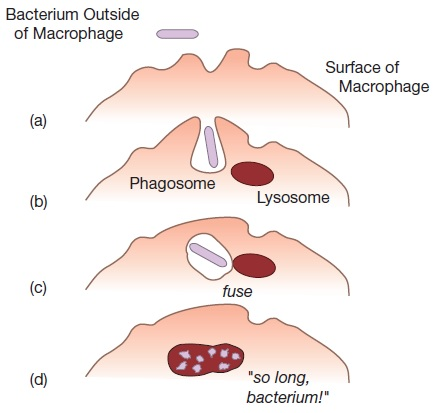
\includegraphics[width=0.5\textwidth]{1_macrofago}
	\caption{Fagocitosis.}
	\label{fig:macrofago}
\end{figure}


Durante la batalla con las bacterias, los \textit{macrófagos} producen y secretan unas proteínas llamadas \textit{citoquinas}.
Estas son hormonas que facilitan la comunicación entre células del sistema inmune y que cobrarán un papel muy relevante en los capítulos que siguen.
Podríamos decir que los \textit{macrófagos} hacen el papel de centinelas, que cuando ven al enemigo mandan señales (\textit{citoquinas}) para reclutar a más defensores. A continuación, veremos otros tipos de células, en este caso referentes al \textit{sistema inmune adaptativo}.

\subsection{El sistema inmune adaptativo}


El nombre es bastante descriptivo y, valga la redundancia, gracias a el somos capaces de adaptar nuestras defensas contra nuevos invasores. Pero no fue hasta los años 70 cuando tuvimos constancia de esta habilidad adaptativa. Por aquel entonces Edward Jenner, conocido como ``el padre de la inmunología'' \footnote{\url{https://historia.nationalgeographic.com.es/a/edward-jenner-probablemente-cientifico-que-mas-vidas-ha-salvado-historia_14242}}, comenzó a vacunar a la población inglesa contra el virus de la viruela, en esa época este virus fue la causa de numerosas muertes y desfiguraciones. Lo que Jenner observó es que los ganaderos que se dedicaban a ordeñar vacas y que contraían el virus de la viruela bovina (\textit{cowpox, en inglés}) raramente contraían la viruela. Así que Jenner decidió llevar a cabo un experimento, poniendo en práctica el método conocido como \textit{variolización} \footnote{Este proceso consistía en inocular material infectado a una persona sana y fue introducido en Londres en 1721 por  Lady Montagu, esposa del embajador inglés en Turquía.} que aprendió en el hospital de San Jorge de Londres: para ello, guardó pus de uno de los ganaderos con viruela bovina y lo usó para inocular a un niño sano, James Phillips. El resultado fue una fiebre leve que desapareció a los pocos días, después Phillips fue reinoculado con pus proveniente de una persona con viruela, pero no contrajo la enfermedad. De esta manera, Jenner demostró que el sistema inmune humano podía proporcionar armas para protegernos de un intruso que no había visto antes, ¡había inventado la vacuna!. Lo que debemos remarcar es que la vacuna contra la viruela solo protegía contra esta enfermedad o algunas causadas por virus similares, como en el caso de la viruela bovina. Es decir, el sistema inmune adaptativo se adapta para defendernos de invasores \textit{específicos}. 

Veamos ahora qué forma tienen estos invasores: seguro que el término \textit{anticuerpo} resulta familiar, pero ¿a qué nos referimos exactamente con él? Los \textit{anticuerpos} no son más que proteínas especiales que circulan por la sangre, y el agente que hace que se produzcan se denomina \textit{antígeno} (en el ejemplo anterior, el \textit{antígeno} sería el virus de la viruela). Gracias a su estructura, los \textit{anticuerpos} son capaces de encajar en un determinado \textit{antígeno}, como vemos en la Figura \ref{fig:macrofago_anticuerpo}. Es decir, los \textit{anticuerpos} son únicos y sirven para defender al organismo de un \textit{antígeno} concreto.

La misión principal de los \textit{anticuerpos} es identificar a los ``indeseables'', dejando que el trabajo sucio lo hagan otros. Es decir, gracias a la presencia de \textit{anticuerpos}, otras células, como los ya conocidos \textit{macrófagos} son capaces de identificar a los atacantes. Pero... ¿qué ocurre cuando un virus ya ha entrado en una célula de nuestro cuerpo? Los \textit{anticuerpos} no pueden alcanzarlo y el virus puede dedicarse a replicarse cuanto quiera. En este momento, es el turno de las células protagonistas de este trabajo, las células T. 


\begin{figure}[t]
	\centering
	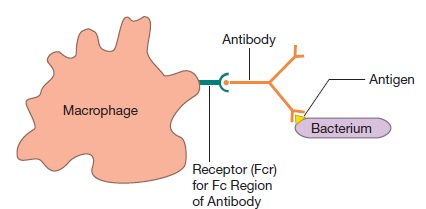
\includegraphics[width=0.5\textwidth]{2_macrofago_anticuerpo}
	\caption{Macrófago reconociendo una bacteria gracias a la acción anticuerpo-antígeno.}
	\label{fig:macrofago_anticuerpo}
\end{figure}


\subsubsection{Las células T}
\label{Tcell}
Al igual que las células B, las células T se producen en la médula y ambas son muy similares en  cuanto a su apariencia, de hecho, con un microscopio ordinario, un inmunólogo no sabría diferenciarlas \citep{theHowItWorks}.  La superficie de las células T también consta de unas moléculas que permiten la interacción con los \textit{anticuerpos} llamados receptores (TCR, \textit{T Cell Receptors}). Estos receptores son de gran importancia, pues son el medio que tienen las células para obtener información de su entorno y poder tomar decisiones en base a ello. Por ejemplo, cuando los receptores de una célula T enlazan con el correspondiente antígeno, las células proliferan para dar lugar a otras con la misma especificidad, es decir, que enlacen con el mismo antígeno. Esta decisión de reproducción, que discutiremos con más detalle en los capítulos que siguen, es específica y lenta, tarda alrededor de una semana en completarse \citep{theHowItWorks}, lo que contrasta con la respuesta rápida que nos ofrecía el \textit{sistema inmune innato}.

Hemos visto algunas de las similitudes que tienen las células B y T. Veamos algunas de sus diferencias: las células T maduran en el timo, de ahí la T de su nombre, mientras que las B maduran en la médula ósea. Además, las células B producen \textit{anticuerpos} que pueden reconocer cualquier molécula orgánica, las células T, por su parte, están especializadas en el reconocimiento de un \textit{antígeno} específico y sus receptores permanecen siempre adheridos a la membrana celular y no pueden ser expulsados en forma de \textit{anticuerpo} como en el caso de las células B.

Hay distintos tipos de células T atendiendo al papel que desempeñan, los tres más importantes son: 
\begin{itemize}
	\item \textit{Killer T-Cells}: su misión es la de reconocer las células que han sido infectadas y, tras este proceso de reconocimiento, las inducen al suicidio. De esta manera muere el virus pero también la célula que había sido infectada por el. Constituyen una de las armas más potentes del sistema inmune.
	
	\item \textit{Helper T-Cells}: se encargan de regular la respuesta inmune. Una de sus tareas principales es secretar \textit{citoquinas} para controlar que la respuesta inmune sea proporcional y las células T no reaccionen de manera exagerada.
	
	\item \textit{Regulatory T-Cells}: estas mantienen la tolerancia a antígenos propios, previniendo la aparición de enfermedades autoinmunes.
\end{itemize}

Cuando las células T salen del timo se encuentran desactivadas, en un estado \textit{naïve} y se dedican a circular por los órganos linfoides secundarios, cuyo máximo representante es el nodo linfático. Allí pueden encontrarse con células provenientes del foco de una infección, que han fagocitado a algún agente infeccioso. Estas presentan en su membrana ciertos \textit{antígenos}, que son reconocidos por las células T gracias a su TCR. Si este \textit{antígeno} se reconoce como extraño, la célula T se activa, convirtiéndose así en una célula efectora, capaz de secretar \textit{citoquinas} o de ir a la zona afectada a combatir al \textit{antígeno} activamente. Una vez que las células han sido activadas, estas comienzan a proliferar masivamente, incrementando la población de células T activadas hasta en un factor de $10^6$ veces, en pocos días, las células pueden pasar por unos 15-20 ciclos de reproducción \citep{JTB}. Este proceso se conoce como \textit{expansión clonal}.

Una vez que las células han sido activadas, se han reproducido dando lugar a clones específicos para un determinado \textit{antígeno} y este ha sido vencido, la mayoría de ellas mueren, restaurando así los niveles de población iniciales. Proceso conocido como \textit{contracción clonal}. Esto tiene sus ventajas y sus inconvenientes: está bien porque no queremos que nuestro organismo conserve demasiadas células T viejas. Sin embargo, sería de gran utilidad tener cerca a alguna de estas células experimentadas cerca para poder reaccionar más rápido en caso de que el mismo invasor vuelva a aparecer. Lo que hace nuestro sistema inmune es mantener un pequeño porcentaje de la población  ($5-10\%$) como células de memoria \citep{JTB}. Se llaman así porque guardan información del \textit{antígeno} contra el que combatieron son más fáciles de activar y nuestro cuerpo puede dar una respuesta inmune más rápidamente.

A lo largo de este trabajo nos centraremos en esta última parte, en el proceso de decisión entre división o suicidio celular de una célula T durante la respuesta inmune. En la sección y los capítulos que siguen veremos cómo se ha abordado este problema, aún desconocido, desde el punto de vista matemático y las conclusiones que se han extraído. 


\section{Cooperación entre dos ciencias: Matemáticas y Biología}

En esta sección trataremos de ver la intersección entre dos ciencias muy distintas: las matemáticas y la biología, y daremos algunos ejemplos de colaboraciones y modelos matemáticos creados para reproducir e investigar distintos procesos biológicos. Nos centraremos en aquellos referidos a las células T, sobre todo al caso que nos ocupa: la dinámica de población de las mismas durante la respuesta inmune.

A pesar de que las matemáticas han influido en investigaciones biológicas muy importantes como los trabajos de Gregor Mendel en genética y los de Theodor Boveri en la naturaleza de los cromosomas (\cite{mathsModInmu}, \cite{esteban2003mendel}), las colaboraciones matemáticas-biología no han sido muy frecuentes. Causa que puede ser justificada por el evidente contraste académico que tienen ambas y que veremos un poco más detalladamente en la sección siguiente. Dediquemos ahora unas líneas a entender por qué los modelos matemáticos son una potente herramienta en el campo de la investigación: un modelo matemático es una máquina lógica que convierte hipótesis en conclusiones. Si el modelo es correcto y las hipótesis son ciertas entonces debemos, por lógica, creer sus conclusiones. Esta garantía lógica permite al matemático que desarrolla el modelo navegar con confianza lejos de las hipótesis y, probablemente, más lejos del lugar al que la intuición permite llegar \citep{Gunawardena2014}. Sin embargo, no debemos confundirnos, los modelos no son respuestas seguras, son, en la mayoría de casos, predicciones que son consecuencia lógica de las hipótesis. En palabras de James Black \footnote{Biografía de este famoso farmacólogo: \url{https://www.britannica.com/biography/James-Black}}, son descripciones precisas de nuestro patético pensamiento (<<\textit{accurate descriptions of our pathetic thinking}>>).

Los modelos son herramientas en las que un biólogo se puede apoyar, pero no todos los modelos son igual de útiles. Veremos las guías que sugiere \cite{Gunawardena2014} para elaborar un buen modelo matemático:

\begin{enumerate}
	\item \textit{Formula una pregunta}. En ocasiones los modelos matemáticos no son diseñados para el avance del conocimiento de la biología, solo responden a investigaciones matemáticas que se basan, aparentemente, en problemas biológicos. Como ya se ha comentado en alguna ocasión, los modelos deben centrarse en aportar información que el biólogo desconocía. Intentar responder con el modelo a una pregunta puede ser clave a la hora de desarrollarlo con criterio, para que pueda ser juzgado por profesionales no matemáticos. 
	
	\item \textit{Hazlo simple}. Incluir todos los procesos bioquímicos puede tranquilizar a los biólogos pero no hará que el modelo sea mejor, de hecho se convertirá en un modelo repleto de parámetros, poco flexible, difícil de estudiar y simular. Es mejor tener unas hipótesis simples y claras, intentando buscar una abstracción del problema.
	
	\item \textit{Si el modelo no puede ser refutado, entonces no está diciendo nada interesante}. No es suficiente con que el modelo reproduzca hechos observados. En muchas ocasiones el ajustar demasiado el modelo provoca que lo seleccionemos para que se ajuste a lo que queremos explicar.  
\end{enumerate}

Podemos distinguir dos tipos de estrategia en cuanto a los modelos se refiere: Modelado hacia adelante (\textit{forward modeling}) o inverso (\textit{reverse modeling}). El modelado inverso empieza con los datos experimentales, construye correlaciones entre ellos y les da estructura con un modelo matemático. Por su parte, el modelado hacia adelante empieza desde lo conocido, o sospechado, expresado en la forma de un modelo, a partir del cual se hacen predicciones. 

El modelado inverso se ha utilizado con el fin de analizar el exceso de datos genómicos y postgenómicos y, a veces, se equipara erróneamente con la biología de sistemas. Ocasionalmente ha sugerido nuevas ideas conceptuales, pero se ha utilizado con mayor frecuencia para sugerir nuevos componentes o interacciones moleculares, que luego han sido confirmados por enfoques biológicos convencionales. Los modelos en sí mismos han tenido menos importancia para comprender el comportamiento del sistema que como un contexto matemático en el que la inferencia estadística se vuelve factible. En contraste, la mayor parte de nuestra comprensión del comportamiento del sistema, como en conceptos como la homeostasis, la retroalimentación, la canalización y el ruido, han surgido del modelado hacia adelante \citep{Gunawardena2014}.

El descubrimiento del microscopio a finales del siglo XVII provocó una revolución en la biología al revelar mundos invisibles y anteriormente desconocidos. Las matemáticas pueden ser interpretadas en la actualidad como un microscopio más general, ya que, pueden revelar mundos invisibles en todo tipo de datos, no solo ópticos. Por ejemplo, la tomografía computarizada puede revelar una sección transversal de una cabeza humana a partir de la densidad de los rayos X sin abrir la cabeza. Charles Darwin tenía razón cuando escribió que las personas con una comprensión \textit{<<de los grandes principios principales de las matemáticas ... parecen tener un sentido adicional>>} \citep{darwin1887life}. Los biólogos de hoy reconocen cada vez más que las matemáticas apropiadas pueden ayudar a interpretar cualquier tipo de datos. En este sentido, las matemáticas son el próximo microscopio de la biología \footnote{\url{https://www.ncbi.nlm.nih.gov/pmc/articles/PMC535574/}}.

\subsection{Modelos matemáticos \textit{versus} inmunología experimental}

Como hemos visto, son algunas las aportaciones que las matemáticas han hecho al campo de la biología. Sin embargo, muchos de las áreas de la biología se han especializado en gran medida. Esto provoca que una mayor cantidad de detalles sea necesaria para entender los conceptos o sistemas que se estudian y que, por tanto, los modelos matemáticos, que tienden a simplificar y a hablar en términos de fórmulas y ecuaciones y, en muchos casos son difíciles de explicar, como en el caso de la inteligencia artificial, hayan sido mirados \textit{con sospecha}. En el área de la inmunología esto no es muy diferente, en \cite{mathsModInmu} se exponen algunas de las razones por las cuales los modelos matemáticos y las inmunología experimental se han mantenido separados:

\begin{enumerate}
	\item El descubrimiento de nuevos agentes y fenómenos del sistema inmune, acompañados de nueva jerga.
	
	\item El avance rápido de la tecnología y la producción de cada vez más datos.
	
	\item El contraste del entorno académico, cultura y terminología de ambas ciencias.
\end{enumerate}

Puede parecer que las dos primeras sugieren un acercamiento entre las dos ciencias. En muchos procesos biológicos, como los dinámicos, la intuición es insuficiente. Por ejemplo, las dinámicas de poblaciones son bastante complicadas de imaginar, mientras que con un modelo podemos obtener una imagen visual muy simple que nos aporte información sobre aspectos conocidos del comportamiento de la población pero también aspectos desconocidos que el modelo predice. Y es que, se debe señalar que, un buen modelo no es aquel que se limita a reproducir hechos observados, sino el que además aporta al biólogo información que no sabe. Es en ese punto donde reside la verdadera cooperación, pues, de otra manera, el modelo constataría como contribución a las matemáticas pero no serviría de nada en el ámbito para el que fue creado, el biológico. Bien es cierto que el hecho de que en los modelos el fondo biológico se diluya viene dado por la razón 3, ambas ciencias son muy distintas: mientras que la biología basa buena parte de su estudio en la experimentación y la observación, los matemáticos se focalizan en el rigor y en la simplicidad de la formulación del problema. Se podría decir que para los biólogos hay demasiada matemática en los modelos y para los matemáticos más puros es insuficiente \citep{RoleOfM}.

A continuación mencionaremos algunos ejemplos en los que los modelos matemáticos han aportado nuevo conocimiento al campo de la inmunología, concretamente al enfocado en el estudio de las conocidas células T. 

\subsubsection{Movimiento de las células T: ¿dirigido o aleatorio?}

En la Sección \ref{Tcell} contamos que las células T interaccionan en los nodos linfáticos con células que presentan antígenos, provenientes de zonas infectadas. Visto desde fuera, el encuentro de una célula T con aquella que presenta el antígeno puede ser como \textit{buscar una aguja en un pajar} \citep{mathsModInmu}. En el siglo XX, se tenía la hipótesis de que las células T eran guiadas a las células que presentaban antígeno por medio de señales (\textit{citoquinas}). 

Una nueva hipótesis surgió a raíz de la publicación de varios artículos: \cite{Miller1869}, \cite{Stoll1873} y \cite{Bousso1876}. Sus imágenes \textit{in vivo} sugerían que el movimiento que seguían las células T era aleatorio, caótico, alejándose así de la hipótesis anterior. Sin embargo, a pesar de que esta nueva hipótesis concordaba con la observación la situación no era tan simple debido al sesgo que se podría introducir en el seguimiento de las células. Por ejemplo, el movimiento dirigido en un medio lleno de obstáculos, como otras células, puede parecer tener cierto carácter aleatorio. La mejor manera de acabar con estos sesgos es usar un modelo matemático que no solo aporte pistas cualitativas sobre los mecanismos a estudiar sino que permita, en aquellos casos donde se dude sobre varias hipótesis, describir cuantitativamente la manera en la que diferentes mecanismos se combinan en el experimento para probar la validación del modelo. 
Varios modelos fueron propuestos, desde los más sencillos hasta algunos más complejos basados en autómatas, donde las células se rigen mediante reglas estocásticas. Es probable que ambos métodos, dirigido y caótico, estén involucrados pero la respuesta aún se desconoce \citep{mathsModInmu}. Se necesitan más iteraciones observación-modelo-predicción-observación para dar con la respuesta, los modelos no pueden ser tratados como una evidencia, sino como una herramienta de investigación.

\subsubsection{Dinámica de las células T. Decisión entre división o apóptosis}

Antes de ver los distintos trabajos que se han realizado en este ámbito, pongámonos en situación. En \ref{Tcell} decíamos que cuando las células T se activan en presencia de un \textit{antígeno} estas comienzan a reproducirse rápidamente para combatir la infección y, una vez superada, muchas de ellas se suicidan restaurando los valores de población iniciales. Es lo que denominábamos como \textit{expansión clonal} y \textit{contracción clonal}. Más aún, los experimentos realizados ponen de manifiesto que la presencia del \textit{antígeno} no es suficiente para desencadenar la decisión de división o apóptosis, las células T activadas continúan reproduciéndose incluso cuando el estímulo (\textit{antígeno}) está ausente y algunas se suicidan aún cuando el la infección persiste \citep{JTB}. Esto es un hecho observado, lo que se desconoce es el mecanismo de decisión por el cual una célula decide dividirse o morir. Varios modelos matemáticos, desarrollados bajo diferentes hipótesis, han sido propuestos para abordar este asunto: por una parte, se ha sugerido que el proceso de activación de las células T en estado naïve desencadena un programa bastante independiente de la estimulación por \textit{antígeno}. Así las cosas, una célula T efectora, por tanto, ya activada, comienza una serie de divisiones, desde un mínimo entre 7 y 10 y un máximo variable (relacionado con la estimulación por \textit{antígeno} que recibe cada célula de manera individual). Después de estas divisiones, la célula se suicida. Bajo esta suposición, la cantidad de antígeno que percibe una célula T en estado naïve durante su activación determina las divisiones de todas sus células hijas. Para hacer este modelo un poco más flexible, se propuso que este programa pudiera estar regulado también mediante \textit{citoquinas} y no solo la presencia de \textit{antígeno}, aunque los detalles no han sido formulados aún \citep{JTB}. Por otro lado, se han propuesto alternativas a este modelo basadas en procesos estocásticos. Esto es, la decisión entre división o apóptosis de una célula T viene determinado por la competición de dos relojes estocásticos. Como ocurría en el caso anterior, los procesos celulares y moleculares específicos para dilucidar que este podría ser el algoritmo de decisión aún están en el aire. 

A continuación presentamos otro modelo, expuesto en \cite{JTB}, cuyas hipótesis biológicas, ecuaciones y simulaciones se desarrollan durante los capítulos siguientes. Es un modelo basado en la acción de dos proteínas inhibidoras, Retinoblastoma (Rb) y célula B linfoma-2 (Bcl-2). Dependiendo de la concentración de estas dos sustancias, la célula tomará la decisión de dividirse o, por el contrario, de suicidarse.  


